\documentclass[usenames,dvipsnames,tikz]{standalone}
\usetikzlibrary{shapes.geometric}
\usepackage{xcolor}
\colorlet{tBlue}{RoyalBlue!35!Cerulean}
\colorlet{tRed}{Red}
\usepackage{tikz}
\usepackage{standalone}
\begin{document}
	
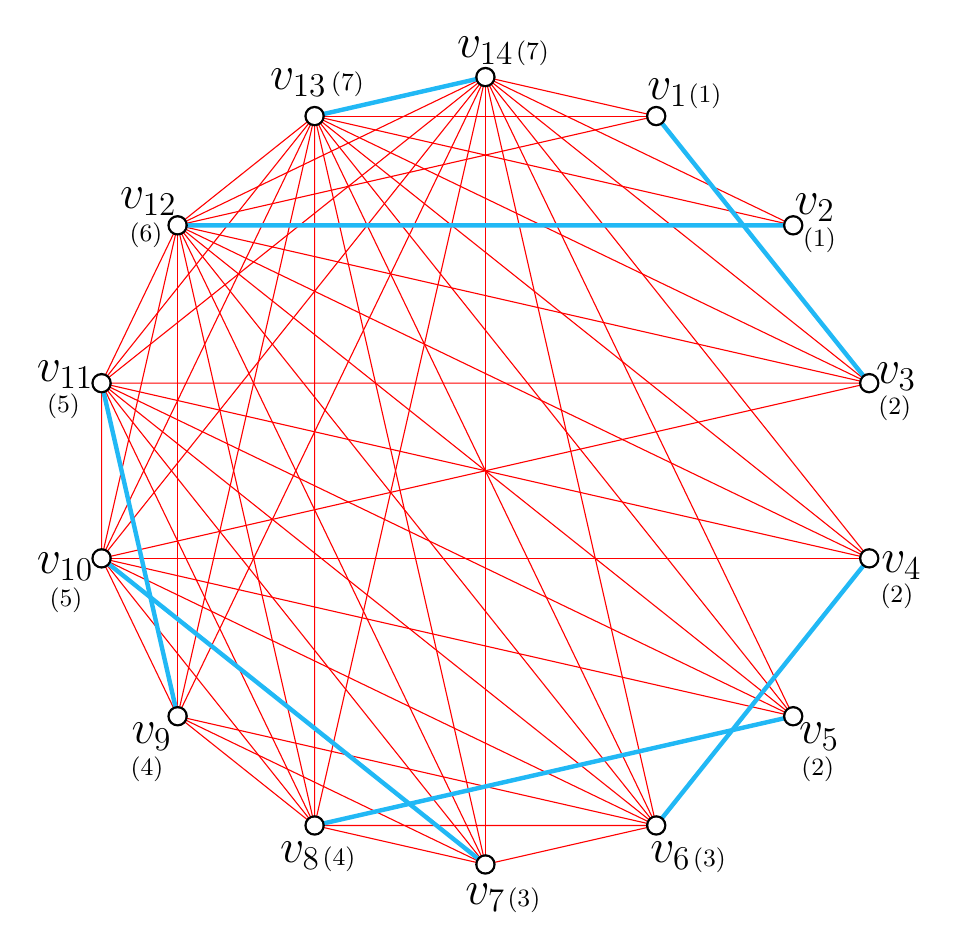
\begin{tikzpicture}
%Values of nodes:
% v1=1, v2=1, v3=2, v4=2, v5=2, v6=3, v7=3, v8=4, v9=4, v10=5, v11=5, v12=6, v13=7, v14=7 (v13/v14 universal vertices), \tau = 7.


\foreach \n/\value in {1/1, 2/1, 3/2, 4/2, 5/2, 6/3, 7/3, 8/4, 9/4, 10/5, 11/5, 12/6, 13/7, 14/7}
	\fill (90-\n*25.71428571:5cm) coordinate (v\n) circle [radius = 0.1];
	
%Labels	
\foreach \n/\value in {1/1, 14/14}
	\fill (90-\n*25.71428571:5cm) coordinate (v\n) circle [radius = 0.1]
		++(90-\n*25.71428571:9.5pt) node {\LARGE{$v_{\value}$}};
		
\foreach \n/\value in {2/2, 3/3}
	\fill (90-\n*25.71428571:5cm) coordinate (v\n) circle [radius = 0.1]
		++(90-\n*25.71428571:10pt) node {\LARGE{$v_{\value}$}};
		
\foreach \n/\value in {4/4, 5/5, 6/6, 7/7, 8/8, 9/9}
	\fill (90-\n*25.71428571:5cm) coordinate (v\n) circle [radius = 0.1]
		++(90-\n*25.71428571:12pt) node {\LARGE{$v_{\value}$}};

\foreach \n/\value in {10/10, 11/11, 12/12, 13/13}
	\fill (90-\n*25.71428571:5cm) coordinate (v\n) circle [radius = 0.1]
		++(90-\n*25.71428571:13.5pt) node {\LARGE{$v_{\value}$}};

%v1
\foreach \n/\value in {1/1}
	\fill (90-\n*25.71428571:5cm) coordinate (v\n) circle [radius = 0.1]
		++(90-\n*68:19pt) node {\small{(\value)}};

%v2		
\foreach \n/\value in {2/1}
	\fill (90-\n*25.71428571:5cm) coordinate (v\n) circle [radius = 0.1]	
		++(90-\n*60:11pt) node {\small{(\value)}};

%v3		
\foreach \n/\value in {3/2}
	\fill (90-\n*25.71428571:5cm) coordinate (v\n) circle [radius = 0.1]
		++(90-\n*45:13pt) node {\small{(\value)}};	

%v4		
\foreach \n/\value in {4/2}
	\fill (90-\n*25.71428571:5cm) coordinate (v\n) circle [radius = 0.1]
		++(90-\n*36:17pt) node {\small{(\value)}};	
	
%v5		
\foreach \n/\value in {5/2}
	\fill (90-\n*25.71428571:5cm) coordinate (v\n) circle [radius = 0.1]
		++(90-\n*31:21pt) node {\small{(\value)}};	
		
%v6		
\foreach \n/\value in {6/3}
	\fill (90-\n*25.71428571:5cm) coordinate (v\n) circle [radius = 0.1]
		++(90-\n*20.5:23pt) node {\small{(\value)}};	
	
%v7		
\foreach \n/\value in {7/3}
	\fill (90-\n*25.71428571:5cm) coordinate (v\n) circle [radius = 0.1]
		++(90-\n*19:19pt) node {\small{(\value)}};
	
%v8		
\foreach \n/\value in {8/4}
	\fill (90-\n*25.71428571:5cm) coordinate (v\n) circle [radius = 0.1]
		++(90-\n*18:15pt) node {\small{(\value)}};	

%v9
\foreach \n/\value in {9/4}
	\fill (90-\n*25.71428571:5cm) coordinate (v\n) circle [radius = 0.1]
		++(90-\n*23.35:22pt) node {\small{(\value)}};		
		
%v10		
\foreach \n/\value in {10/5}
	\fill (90-\n*25.71428571:5cm) coordinate (v\n) circle [radius = 0.1]
		++(90-\n*22:20pt) node {\small{(\value)}};		
	
%v11		
\foreach \n/\value in {11/5}
	\fill (90-\n*25.71428571:5cm) coordinate (v\n) circle [radius = 0.1]
		++(90-\n*21.75:16pt) node {\small{(\value)}};	
	
%v12		
\foreach \n/\value in {12/6}
	\fill (90-\n*25.71428571:5cm) coordinate (v\n) circle [radius = 0.1]
		++(90-\n*21:12pt) node {\small{(\value)}};		
	
%v13		
\foreach \n/\value in {13/7}
	\fill (90-\n*25.71428571:5cm) coordinate (v\n) circle [radius = 0.1]
		++(90-\n*31.25:16.5pt) node {\small{(\value)}};		
		
%v14		
\foreach \n/\value in {14/7}
	\fill (90-\n*25.71428571:5cm) coordinate (v\n) circle [radius = 0.1]
		++(90-\n*30.25:19pt) node {\small{(\value)}};			
							
%Edges and vertices
\foreach \m/\n in {1/12, 1/13, 1/14, 2/13, 2/14, 3/10, 3/11, 3/12, 3/13, 3/14, 4/10, 4/11, 4/12, 4/13, 4/14, 5/10, 5/11, 5/12, 5/13, 5/14, 6/7, 6/8, 6/9, 6/10, 6/11, 6/12, 6/13, 6/14, 7/8, 7/9, 7/11, 7/12, 7/13, 7/14, 8/9, 8/10, 8/11, 8/12, 8/13, 8/14, 9/10, 9/12, 9/13, 9/14, 10/11, 10/12, 10/13, 10/14, 11/12, 11/13, 11/14, 12/13, 12/14}
	\draw [tRed] (v\n) -- (v\m);
\foreach \m/\n in {1/3, 2/12, 4/6, 5/8, 7/10, 9/11, 13/14}
	\draw [ultra thick, tBlue] (v\n) -- (v\m);
\foreach \n in {1,...,14}
	\fill (90-\n*25.71428571:5cm) coordinate (v\n) circle [radius = 0.13];
\foreach \n in {1,...,14}
	\fill [white] (90-\n*25.71428571:5cm) coordinate (v\n) circle [radius = 0.1];

\end{tikzpicture}
	
\end{document}